\documentclass[10pt]{exam}
\usepackage[phy]{template-for-exam}
\usepackage{tikz}

\title{Momentum \#3}
\author{Rohrbach}
\date{\today}

\begin{document}
\maketitle

\begin{questions}
  
  \question
    In a NERF war, a foam dart with a mass of 0.13 kg is shot out of the gun at 3.5 m/s. If the gun has a mass of 1.8 kg, with what velocity does it recoil?
    \vs

  \question
    A soccer player applies a force of 270 N for 0.05 s. to a 0.434-kg ball initially at rest.  What is its final velocity of the ball?
    \vs

  \pagebreak
  
  \question
    A small car with a mass of 800 kg is driving eastwith a velocity of 32 m/s, rear-ends a 1300 kg microbus also traveling east with a velocity of 10 m/s. If the small car has a final velocity of 18 m/s, what is the final velocity of the microbus?
    \vs
    
  \question
    {\bf Challenge:} A truck with a mass of 5000 kg is traveling \emph{north} with a velocity of 13 m/s. At an intersection, it collides with a car (m = 1500 kg) traveling \emph{east} with a velocity of 20 m/s. What is the velocity of the vehicles after the collision?  Assume they stick together after the crash.
    
    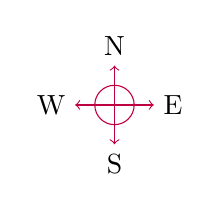
\begin{tikzpicture}[scale=0.5,draw=purple]
      \draw[<->] 
        (1,0) node[right] {E} 
        -- (-1,0) node[left] {W};
      \draw[<->]
        (0,1) node[above] {N} 
        -- (0,-1) node[below] {S};
      \draw (0,0) circle (0.5);

    \end{tikzpicture}

    \vs
  

\end{questions}

\end{document}